\documentclass[9pt,twoside]{pnas-new}
% Use the lineno option to display guide line numbers if required.

\templatetype{pnasmathematics} % Choose template
% {pnasresearcharticle} = Template for a two-column research article
% {pnasmathematics} %= Template for a one-column mathematics article
% {pnasinvited} %= Template for a PNAS invited submission

\begin{document}


\title{Carbon sequestration trade-off between carbon assimilation and carbon losses through respiration and disturbances}

% Use letters for affiliations, numbers to show equal authorship (if applicable) and to indicate the corresponding author
\author[a,b,1]{Estefanía Muñoz}
\author[b]{Author Two}
\author[b]{Author Two}
\author[b]{Carlos A. Sierra}

% Marcos Fernández-Martínez
% Holger Metzler
% Jacob A. Nelson
% Mike O'Sullivan
% Stephan Sitch
% Sophia Walthe



\affil[a]{CREAF, Cerdanyola del Vallès, Barcelona, Catalonia, Spain}
\affil[b]{Theoretical Ecosystem Ecology Group, Max Planck Institute for Biogeochemistry, Jena, Germany}
\affil[c]{Affiliation Three}

% Please give the surname of the lead author for the running footer
\leadauthor{Muñoz}


% Please include corresponding author, author contribution and author declaration information
%\authorcontributions{Please provide details of author contributions here.}
%\authordeclaration{Please declare any competing interests here.}
%\equalauthors{\textsuperscript{1}A.O.(Author One) contributed equally to this work with A.T. (Author Two) (remove if not applicable).}
\correspondingauthor{\textsuperscript{1}Estefanía Muñoz. E-mail: e.munoz\@creaf.uab.cat}

% At least three keywords are required at submission. Please provide three to five keywords, separated by the pipe symbol.
\keywords{Keyword 1 $|$ Keyword 2 $|$ Keyword 3 $|$ ...}





\maketitle
\thispagestyle{firststyle}


\firstpage{2}
% Use \firstpage to indicate which paragraph and line will start the second page and subsequent formatting. In this example, there are a total of 11 paragraphs on the first page, counting the first level heading as a paragraph. The value {12} represents the number of the paragraph starting the second page. If a paragraph runs over onto the second page, include a bracket with the paragraph line number starting the second page, followed by the paragraph number in curly brackets, e.g. "\firstpage[4]{11}".


% If your first paragraph (i.e. with the \dropcap) contains a list environment (quote, quotation, theorem, definition, enumerate, itemize...), the line after the list may have some extra indentation. If this is the case, add \parshape=0 to the end of the list environment.
\renewcommand{\figurename}{Supplementary Figure}
\setcounter{figure}{0}

\renewcommand{\tablename}{Supplementary Table}
\setcounter{table}{0}


\section*{Model information of CMIP6 and TRENDY}


\begin{table}[ht]
\centering
\label{Tab:CMIP6models}
\caption{CMIP6 Earth system models included in this study and relevant features.}
\begin{tabular}{llcccccl}
\textbf{\begin{tabular}[c]{@{}l@{}}Earth system\\  model\end{tabular}} & \textbf{\begin{tabular}[c]{@{}l@{}}Modelling \\ centre\end{tabular}} & \multicolumn{1}{l}{\textbf{NPP}} & \multicolumn{1}{l}{\textbf{NPB}} & \multicolumn{1}{l}{\textbf{N cycle}}                     & \multicolumn{1}{l}{\textbf{Fires}}                       & \multicolumn{1}{l}{\textbf{\begin{tabular}[c]{@{}l@{}}Dynamic \\ vegetation\end{tabular}}} & \textbf{\begin{tabular}[c]{@{}l@{}}Land carbon\\ model\end{tabular}} \\ \hline
ACCESS-ESM1-5                                                          & CSIRO                                                                & Yes                              & Yes                              & \begin{tabular}[c]{@{}c@{}}Yes \\ (p-cycle)\end{tabular} & No                                                       & No                                                                                         & \begin{tabular}[c]{@{}l@{}}CABLE2.4 with\\ CASA-CNP\end{tabular}     \\
BCC-CSM2-MR                                                            & BCC                                                                  & Yes                              & No                               & No                                                       & No                                                       & No                                                                                         & BCC-AVIM2                                                            \\
CanESM5                                                                & CCCma                                                                & Yes                              & Yes                              & No                                                       & No                                                       & \begin{tabular}[c]{@{}c@{}}Only\\ wetlands\end{tabular}                                    & CLASS-CTEM                                                           \\
CESM2                                                                  & CESM                                                                 & No                               & Yes                              & Yes                                                      & Yes                                                      & Yes                                                                                        & CLM5                                                                 \\
CNRM-ESM2-1                                                            & CNRM                                                                 & Yes                              & Yes                              & Implicit                                                 & \begin{tabular}[c]{@{}c@{}}Yes \\ (Natural)\end{tabular} & No                                                                                         & ISBA-CTRIP                                                           \\
NOAA-GFDL-ESM4                                                         & \begin{tabular}[c]{@{}l@{}}NOAA, \\ GFDL\end{tabular}                & Yes                              & Yes                              & No                                                       & Yes                                                      & Yes                                                                                        & LM4p1                                                                \\
MPI-ESM1-2-LR                                                          & MPI                                                                  & Yes                              & Yes                              & Yes                                                      & Yes                                                      & Yes                                                                                        & JSBACH3.2                                                            \\
NorESM2-LM                                                             & NCC                                                                  & Yes                              & Yes                              & Yes                                                      & Yes                                                      & No                                                                                         & CLM5                                                                 \\
UKESM1-0-LL                                                            & UK                                                                   & Yes                              & Yes                              & Yes                                                      & No                                                       & Yes                                                                                        & JULES-ES1.0                                                          \\ \hline
\end{tabular}
\end{table}


\begin{table}[ht]
\centering
\label{Tab:TRENDYmodels}
\caption{TRENDY models included in this study and relevant features.}
\begin{tabular}{llll}
\textbf{Model} & \textbf{NEP} & \textbf{NBP} & \textbf{Reference}                                                                                                                  \\ \hline
CABLE-POP      & Yes          & Yes          & Haverd et al. (2018)                                                                                                                \\
CLASSIC        & Yes          & Yes          & Melton et al. (2020)                                                                                                                \\
CLM5.0         & Yes          & Yes          & Lawrence et al. (2019)                                                                                                              \\
DLEM           & Yes          & No           & Tian et al. (2015), You et al. (2022)                                                                                               \\
ED             & Yes          & Yes          & Moorcroft et al. (2001), Ma et al. (2022)                                                                                           \\
ELM            & Yes          & Yes          & Yang et al.(2023), Burrows et al. (2020)                                                                                            \\
IBIS           & Yes          & Yes          & Xia et al. (2024)                                                                                                                   \\
iMAPLE         & Yes          & Yes          & Yue et al. (2024)                                                                                                                   \\
ISAM           & Yes          & Yes          & \begin{tabular}[c]{@{}l@{}}Jain et al. (2013), Meiyappan et al. (2015), \\ Shu et al. (2020)\end{tabular}                           \\
ISBACTRIP      & Yes          & Yes          & Delire et al. (2020)                                                                                                                \\
JSBACH         & Yes          & Yes          & Mauritsen et al. (2019), Reick et al. (2021)                                                                                        \\
JULES          & Yes          & Yes          & \begin{tabular}[c]{@{}l@{}}Wiltshire et al. (2021), Sellar et al. (2019), \\ Burton et al. (2019)\end{tabular}                      \\
LPJml          & Yes          & No           & \begin{tabular}[c]{@{}l@{}}Schaphoff et al. (2018), von Bloh et al. (2018),\\ Lutz et al. (2019), Heinke et al. (2023)\end{tabular} \\
LPJwsl         & Yes          & Yes          & Poulter et al. (2011)                                                                                                               \\
LPX            & Yes          & Yes          & Lienert and Joos (2018)                                                                                                             \\
OCN            & Yes          & Yes          & Zaehle and Friend (2010), Zaehle et al. (2011)                                                                                      \\
ORCHIDEE       & Yes          & Yes          & \begin{tabular}[c]{@{}l@{}}Krinner et al. (2005), Zaehle and Friend (2010), \\ Vuichard et al. (2019)\end{tabular}                  \\
SDGVM          & Yes          & No           & Woodward and Lomas (2004), Walker et al. (2017)                                                                                     \\
VISIT          & Yes          & Yes          & Ito and Inatomi (2012), Kato et al. (2013)                                                                                          \\
VISIT-UT       & Yes          & Yes          &                                                                                                                                     \\ \hline
\end{tabular}
\end{table}

\newpage
\section*{Model weights}

\begin{figure}[ht!]
    \centering
    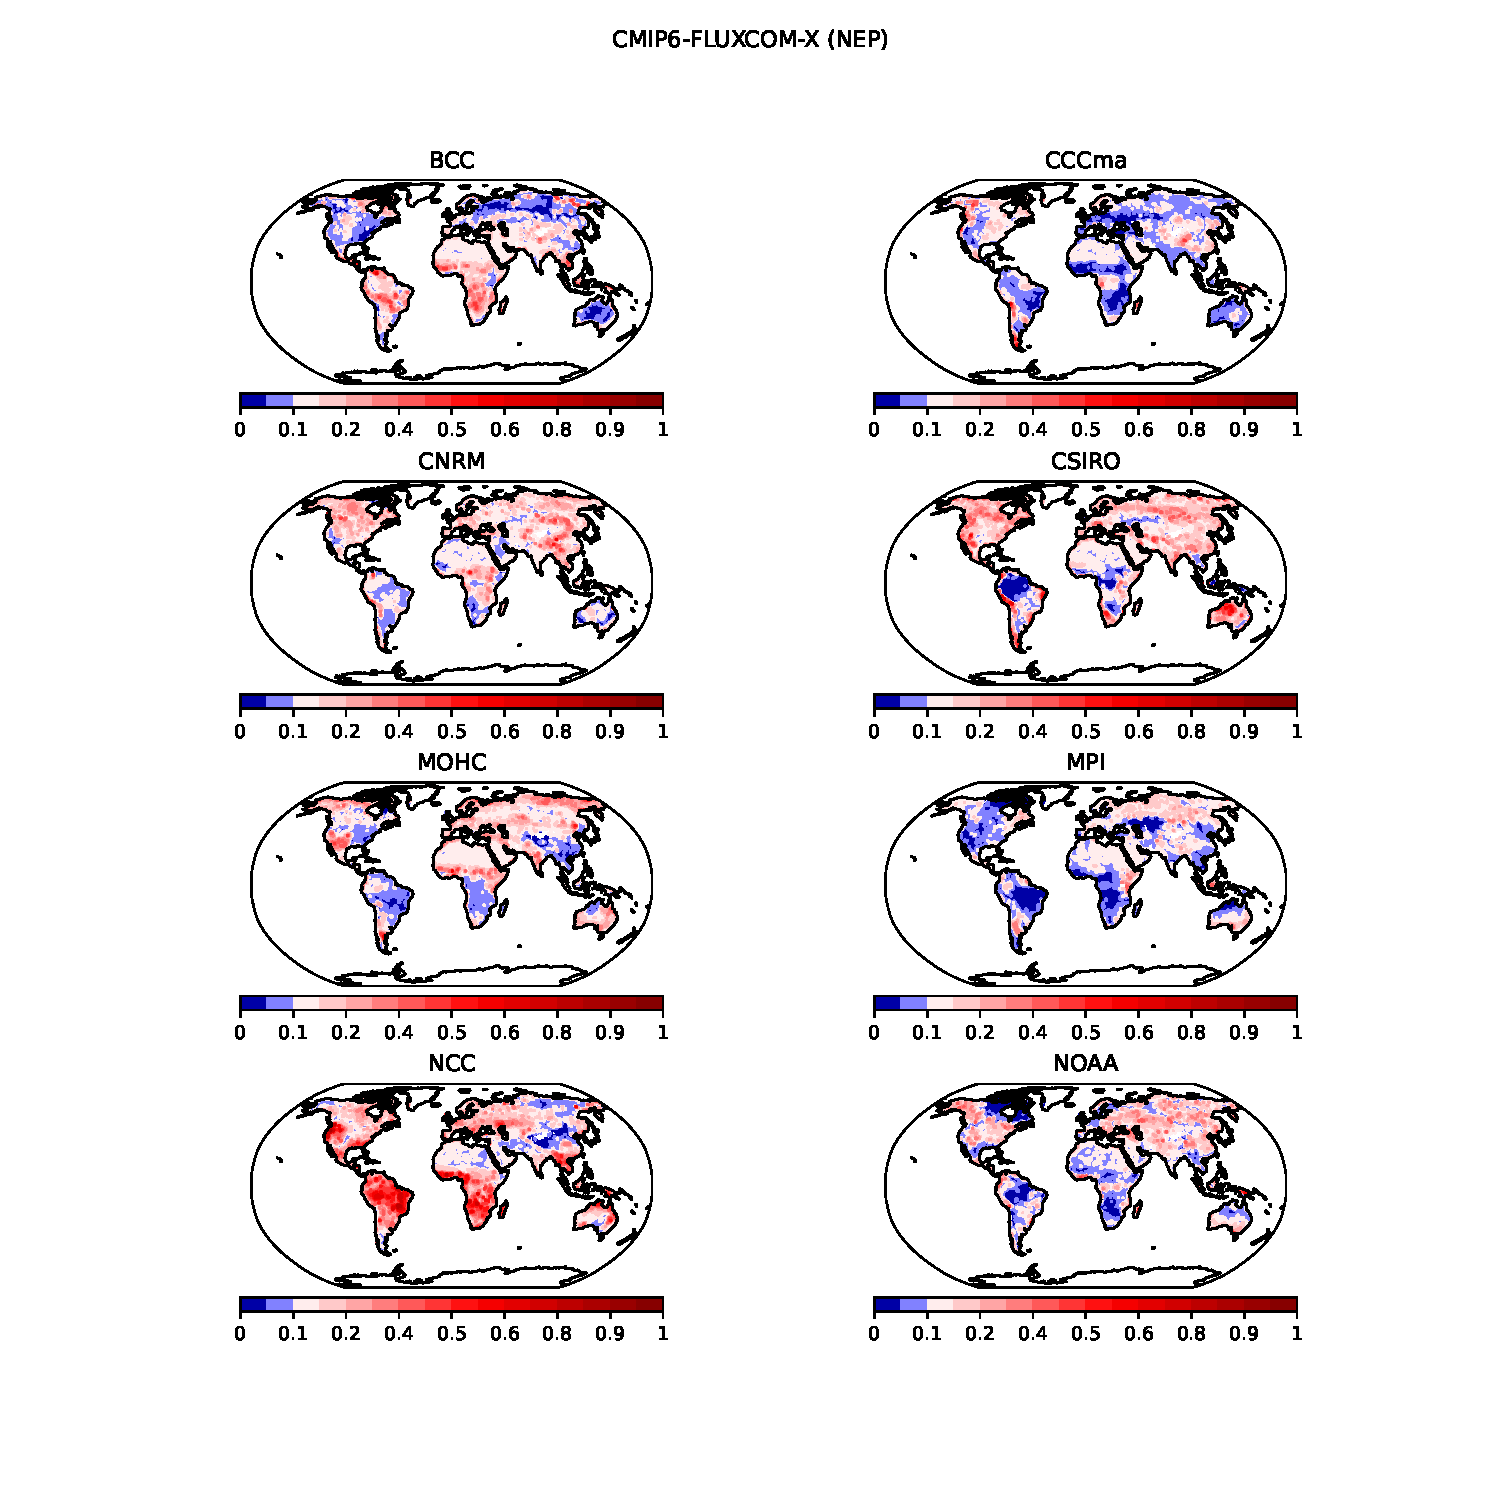
\includegraphics[width=1.0\linewidth]{CMIP6_FLUXCOM_weights.pdf}
    \caption{Spatial weights of NEP CMIP6 models to calculate the ensemble model derived from FLUXCOM-X (NEE). Diverging color tables indicate whether the model contributes more or less than 1/8, where 8 is the number of models.}
    \label{fig:weights_CMIP6-FLUXCOMX}
\end{figure}

\newpage
\begin{figure}[ht!]
    \centering
    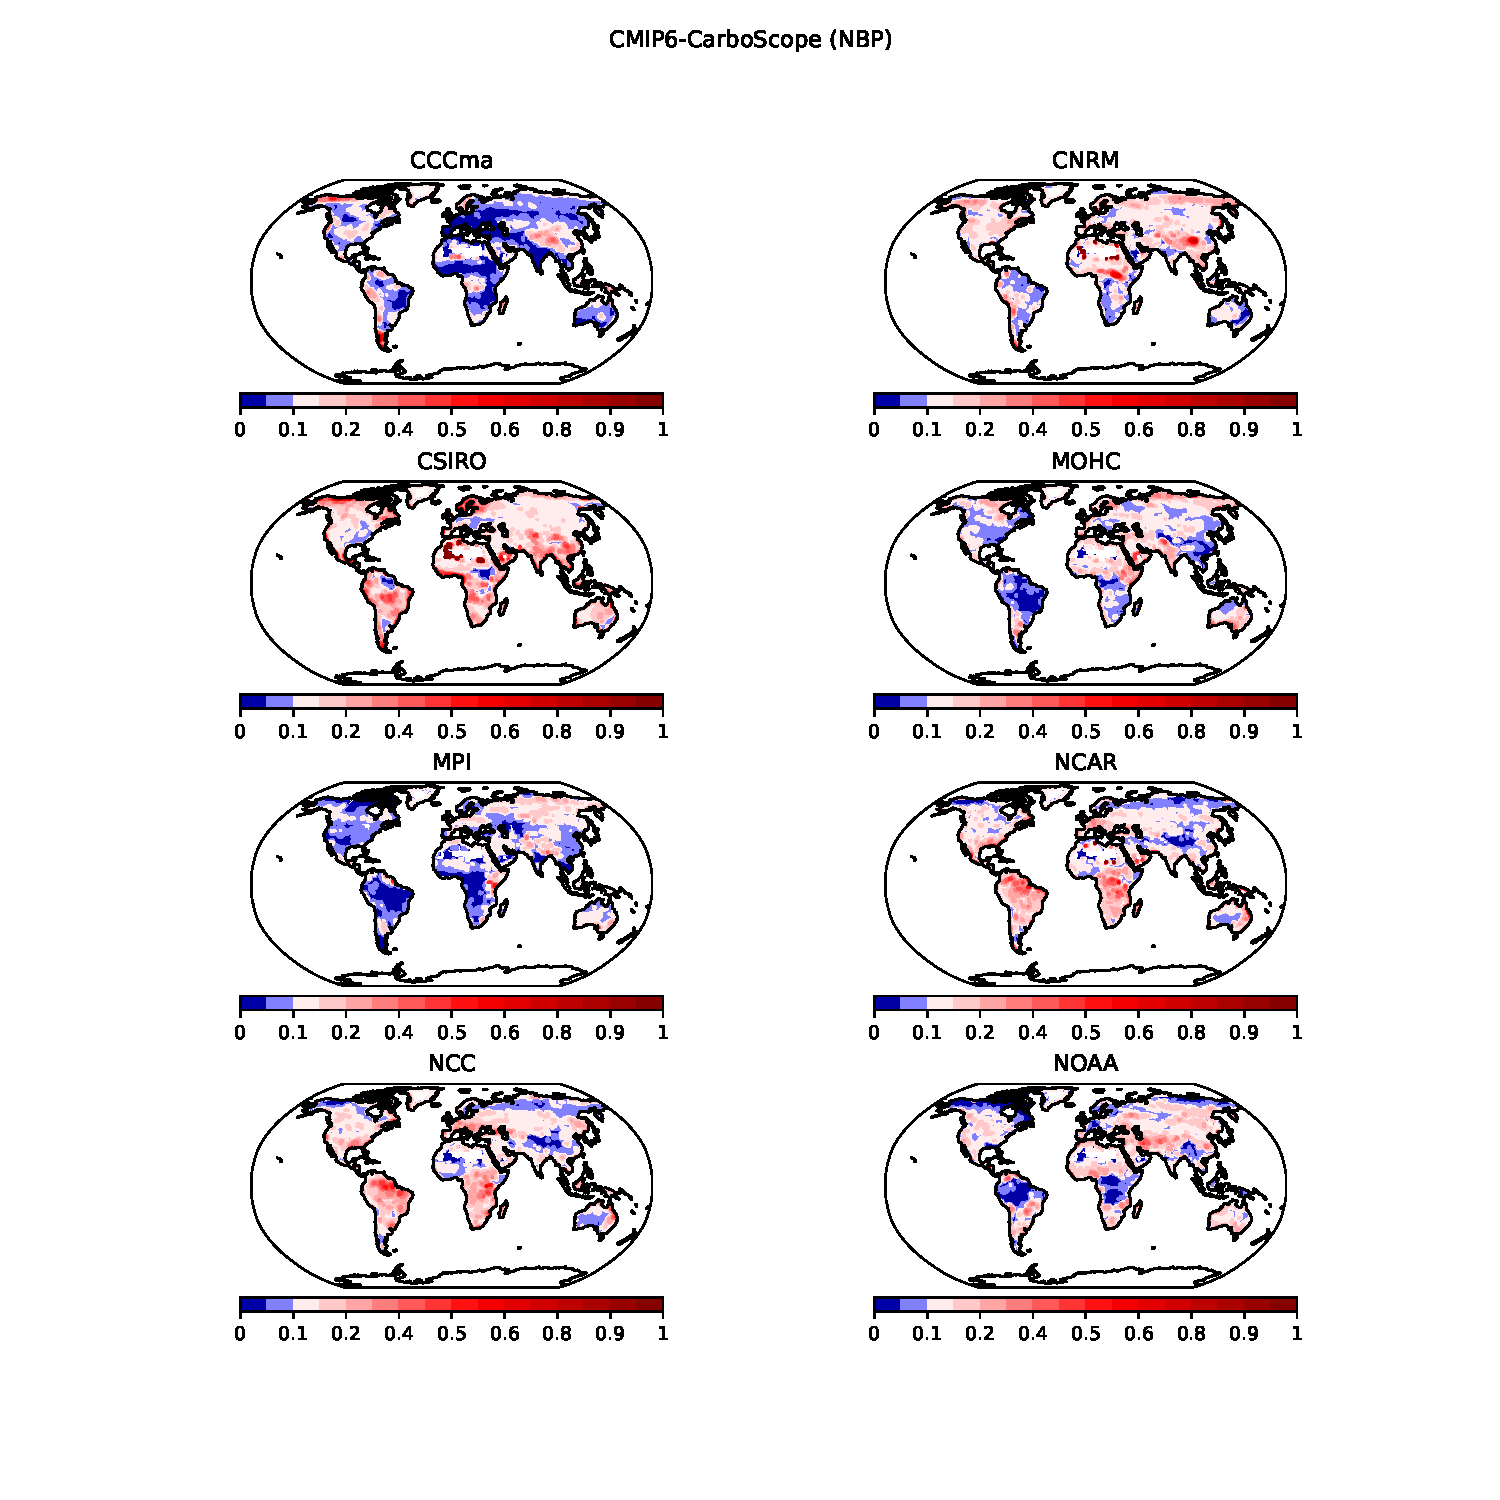
\includegraphics[width=1.0\linewidth]{CMIP6_CarboScope_weights.pdf}
    \caption{Spatial weights of NBP CMIP6 models to calculate the ensemble model derived from CarboScope. Diverging color tables indicate whether the model contributes more or less than 1/8, where 8 is the number of models.}
    \label{fig:weights_CMIP6-CarboScope}
\end{figure}

\newpage
\begin{figure}[ht!]
    \centering
    \includegraphics[width=1.0\linewidth]{TRENDY_FLUXCOM_weights.pdf}
    \caption{Spatial weights of NEP TRENDY models to calculate the ensemble model derived from FLUXCOM-X (NEE). Diverging color tables indicate whether the model contributes more or less than 1/20, where 20 is the number of models.}
    \label{fig:weights_TRENDY-FLUXCOMX}
\end{figure}

\newpage
\begin{figure}[H]
    \centering
    \includegraphics[width=1.0\linewidth]{TRENDY_CarboScope_weights.pdf}
    \caption{Spatial weights of NBP TRENDY models to calculate the ensemble model derived from CarboScope. Diverging color tables indicate whether the model contributes more or less than 1/18, where 18 is the number of models.}
    \label{fig:weights_TRENDY-CarboScope}
\end{figure}

\newpage
\section*{Supplementary figures}

\begin{figure}[h]
    \centering
    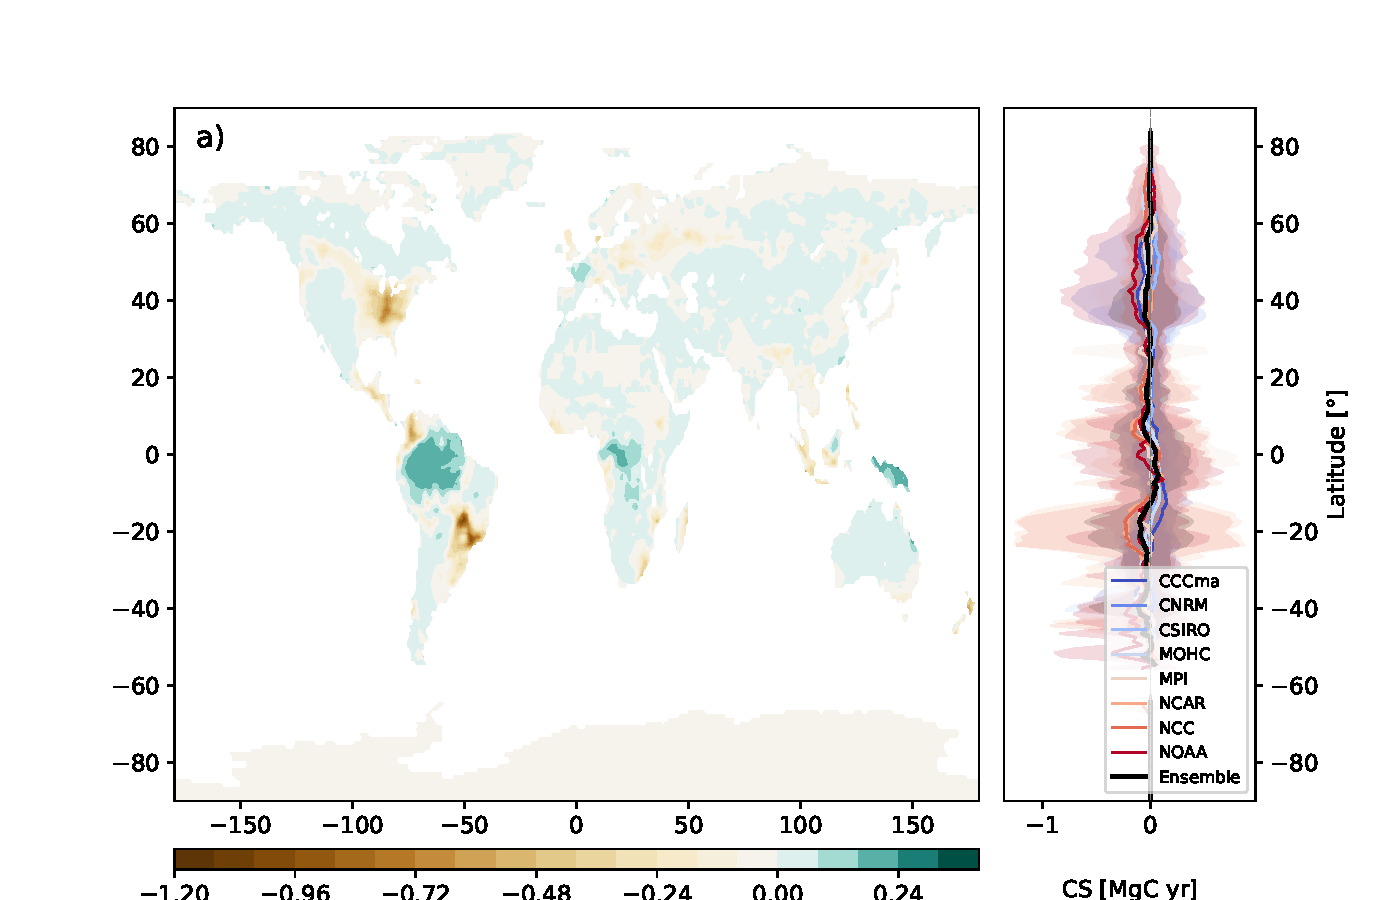
\includegraphics[width=1.0\linewidth]{CMIP6_NBP_CS_map_latitude_mean.pdf}
    \caption{Carbon Sequestration (CS) spatial patterns from NBP from CMIP6 models (1850-2014). a) Global distributions of CS based on the weighted ensemble of 8 CMIP6 models, and b) latitudinal CS profiles for individual CMIP6 models (colored lines) and their ensemble (black line). The dotted line represents zero carbon sequestration and the shadow areas represent two standard deviations from the mean.}
    \label{fig:CMIP6_NBP_map}
\end{figure}

\begin{figure}
    \centering
    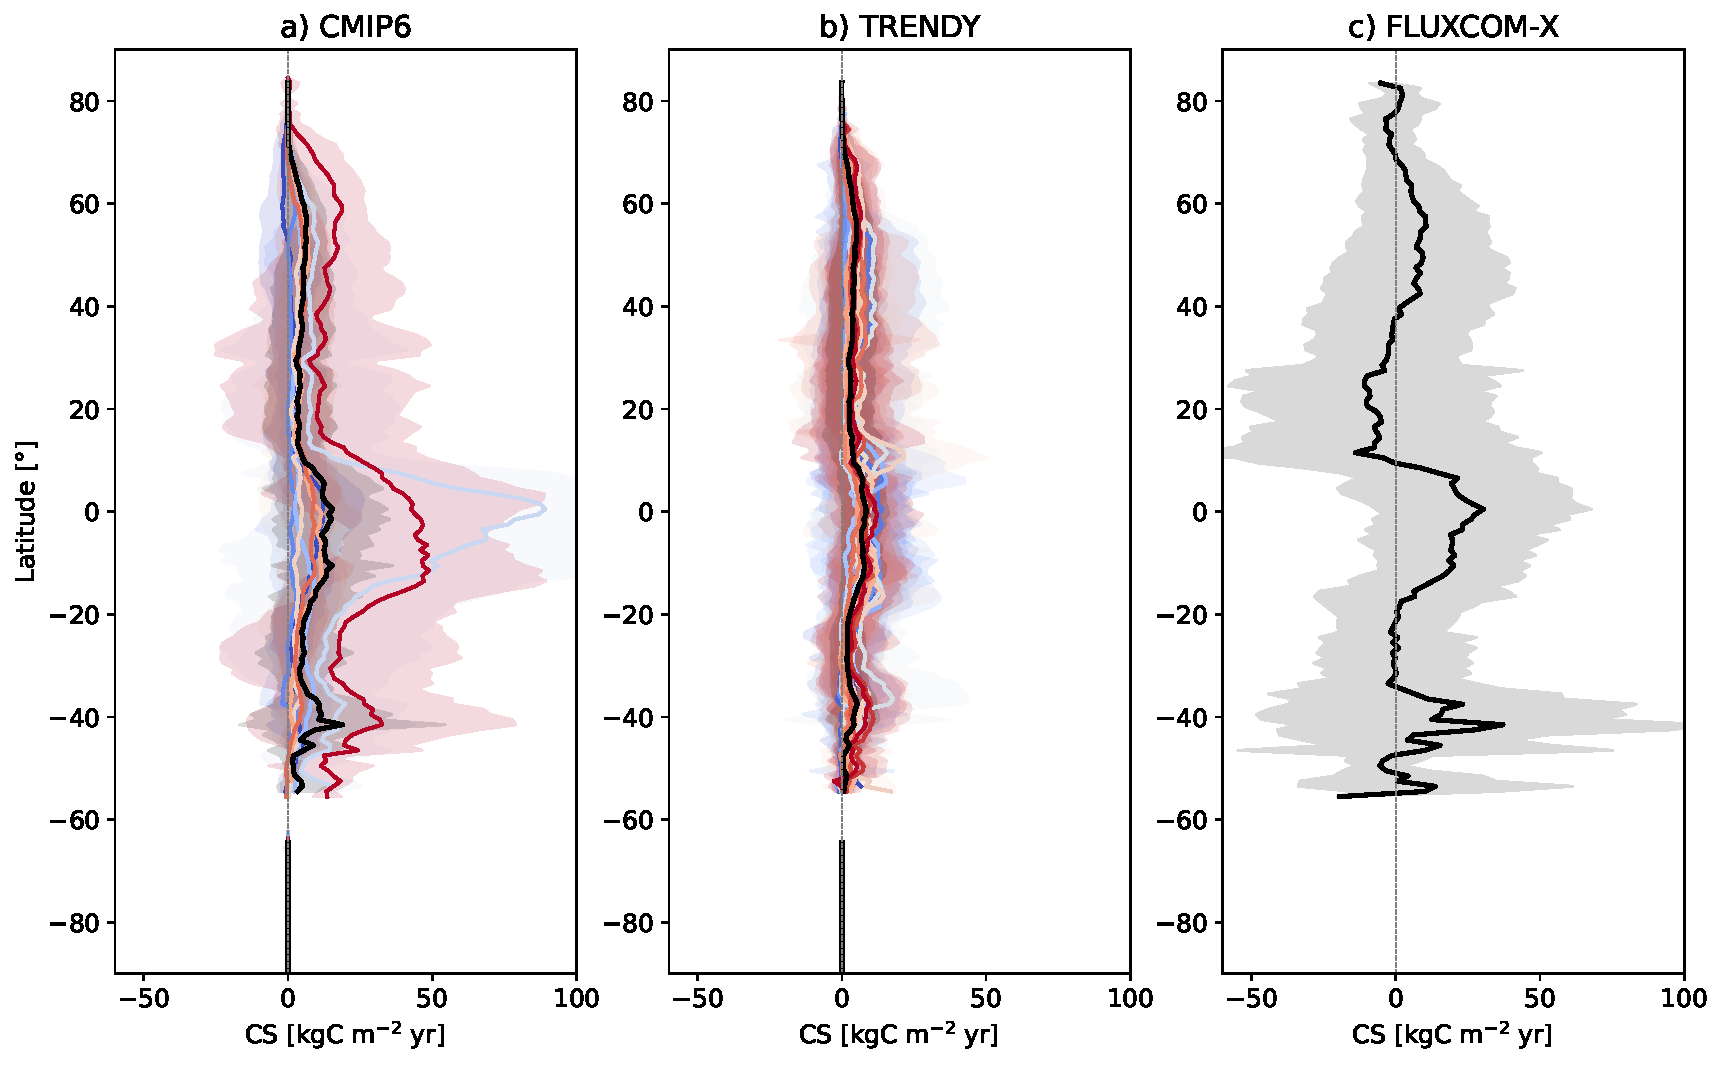
\includegraphics[width=1.0\linewidth]{Comparison_CS_latitude_NEP.pdf}
    \caption{Latitudinal CS profiles obtained from NEP (or NEE) from a) CMIP6, b) TRENDY, and c) FLUXCOM-X. Colored lines in a) and b) represent individual models; the black line is their ensemble. The dotted lines represent null carbon sequestration and the shadow areas two standard deviations from the mean.}
    \label{fig:LatCS_NEP}
\end{figure}

\begin{figure}
    \centering
    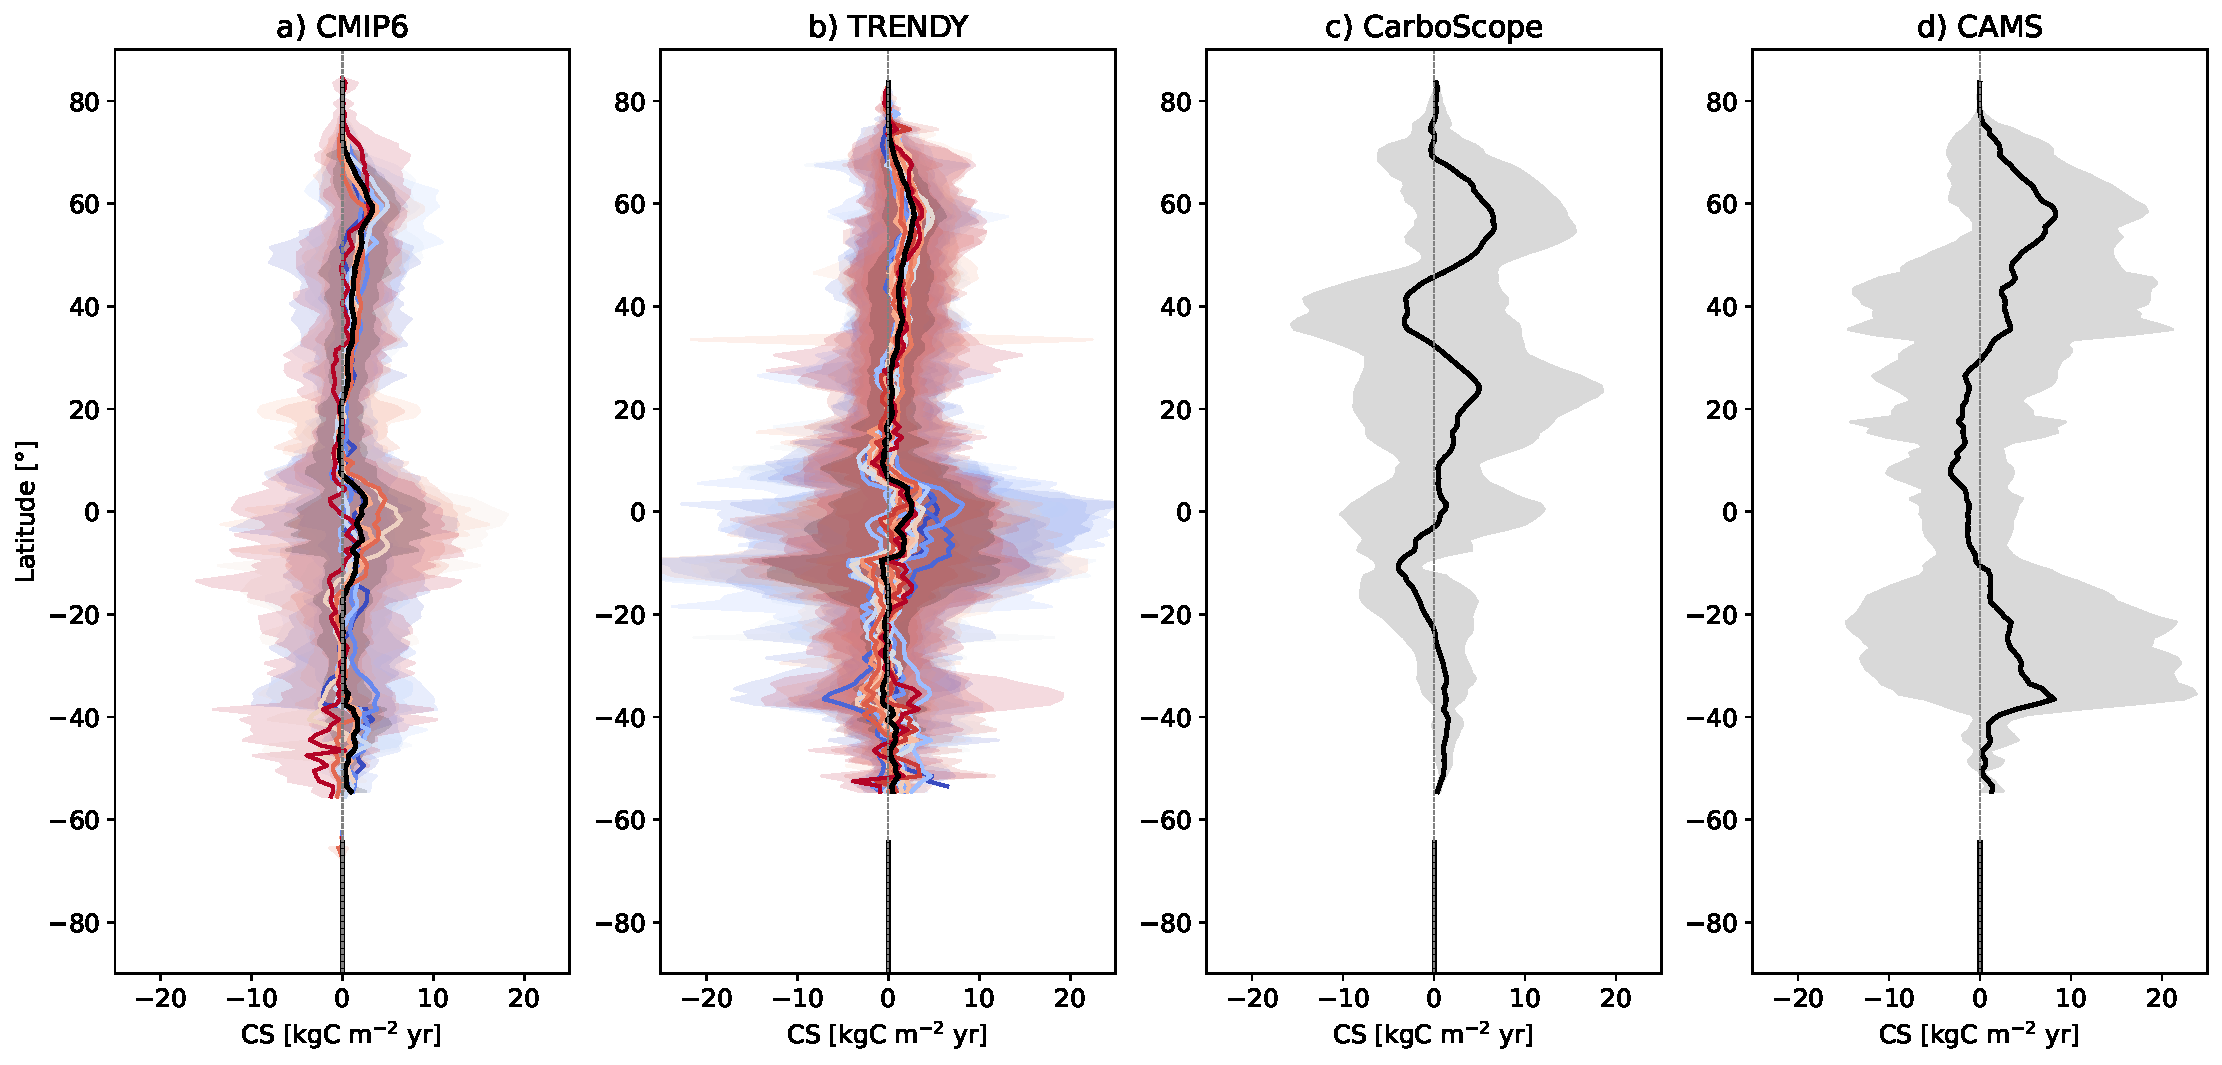
\includegraphics[width=1.0\linewidth]{Comparison_CS_latitude_NBP.pdf}
    \caption{Latitudinal CS profiles obtained from NBP from a) CMIP6, b) TRENDY, c) CarboScope, and d) CAMS. Colored lines in a) and b) represent individual models; the black line is their ensemble. The dotted lines represent null carbon sequestration and the shadow areas two standard deviations from the mean.}
    \label{fig:LatCS_NBP}
\end{figure}

\begin{figure}
    \centering
    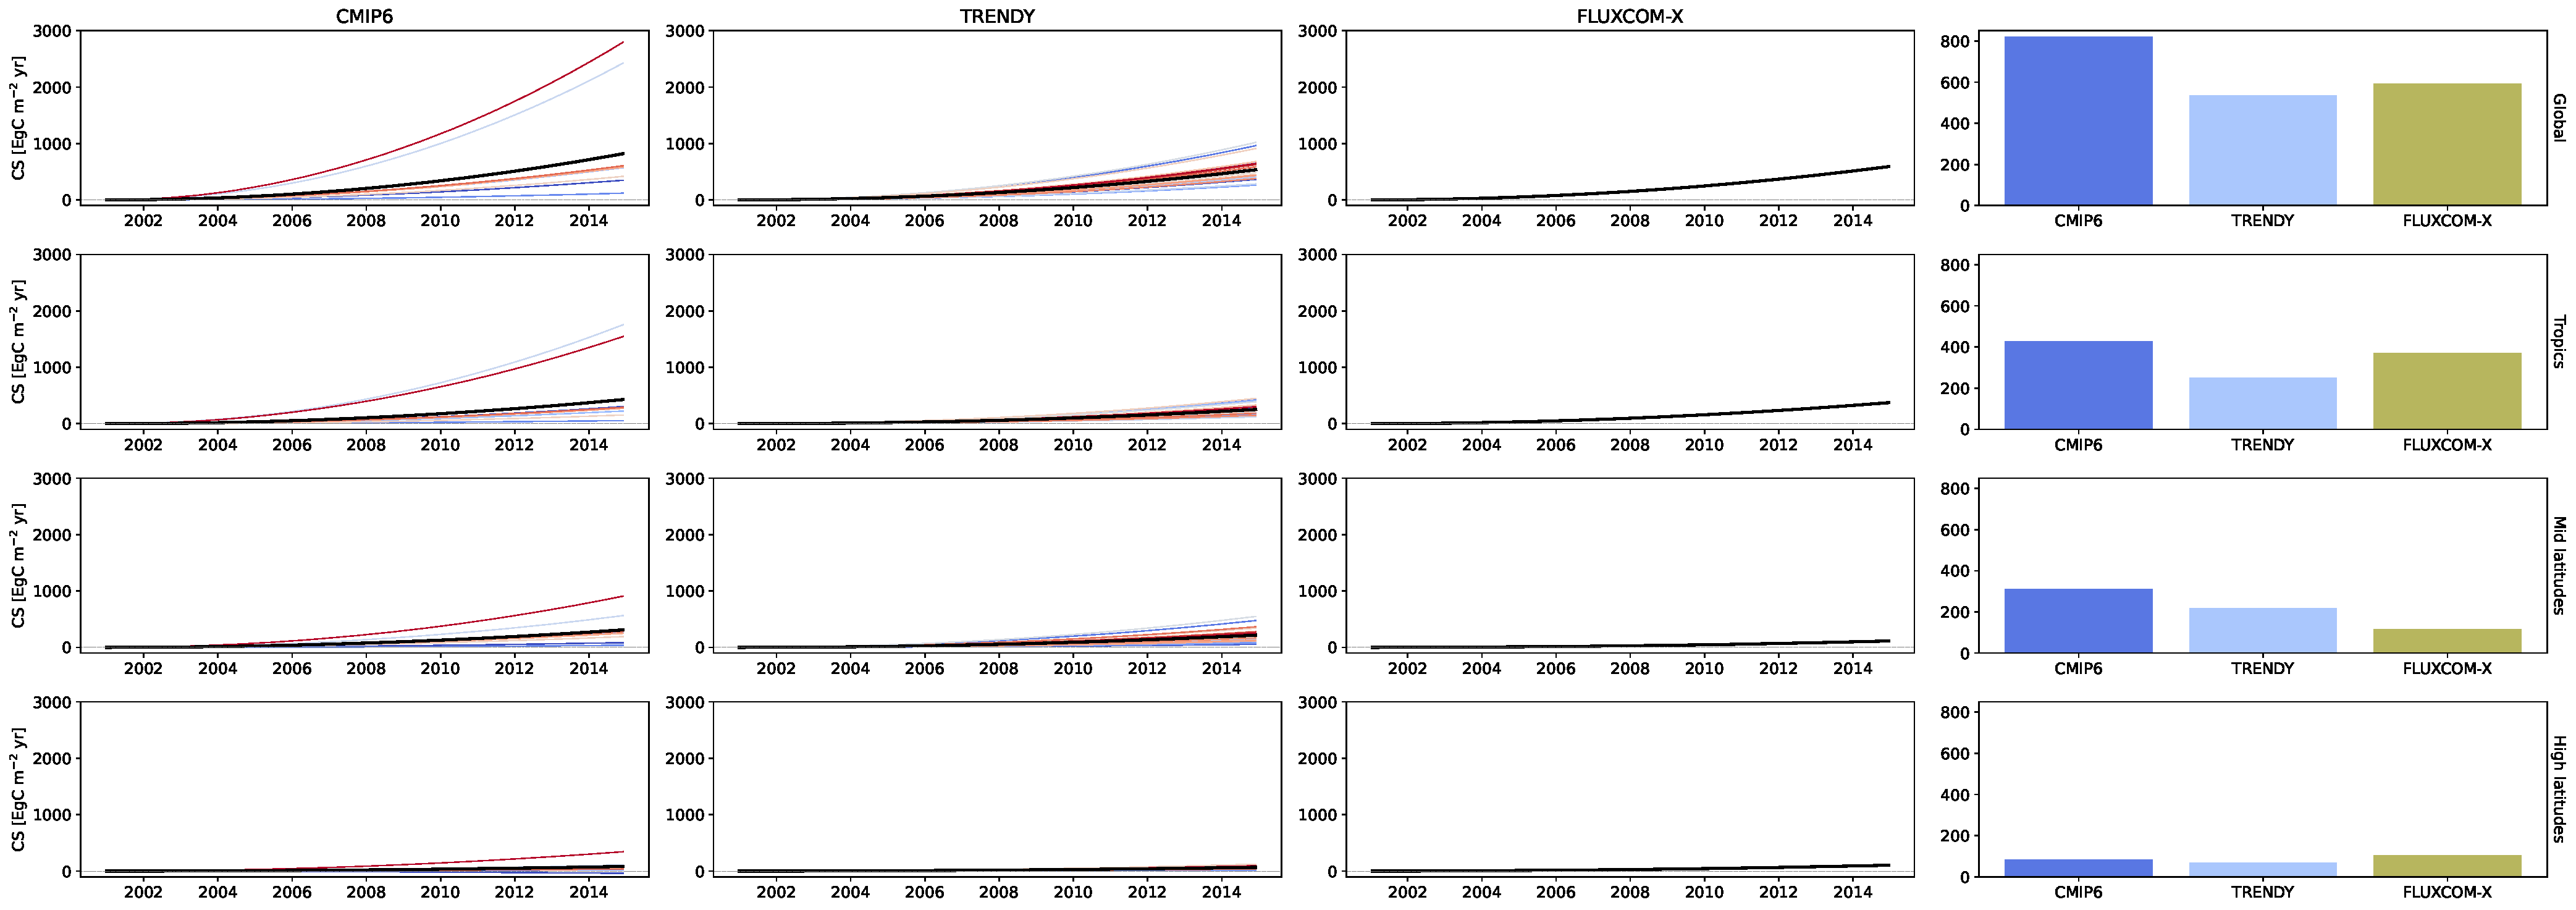
\includegraphics[width=1.0\linewidth]{Comparison_CS_temporal_NEP.pdf}
    \caption{Time accumulation of Carbon Sequestration (CS) of CMIP6 (1st vertical panel), TRENDY (2nd vertical panel), and FLUXCOM-X (3rd vertical panel), and CS at the end of the period from 2001 to 2014 (right panel) calculated using NEP (or NEE) for global (1st horizontal panel), tropics (2nd horizontal panel), mid-latitudes (3rd horizontal panel), and high-latitudes zones (4th horizontal panel). Black lines in 1st and 2nd horizontal panels indicate the results using the ensemble of the models and bars for CMIP6 and TRENDY in the right panel correspond to their ensembles. The dotted lines indicate null values of CS.}
    \label{fig:TempCS_NEP}
\end{figure}

\begin{figure}
    \centering
    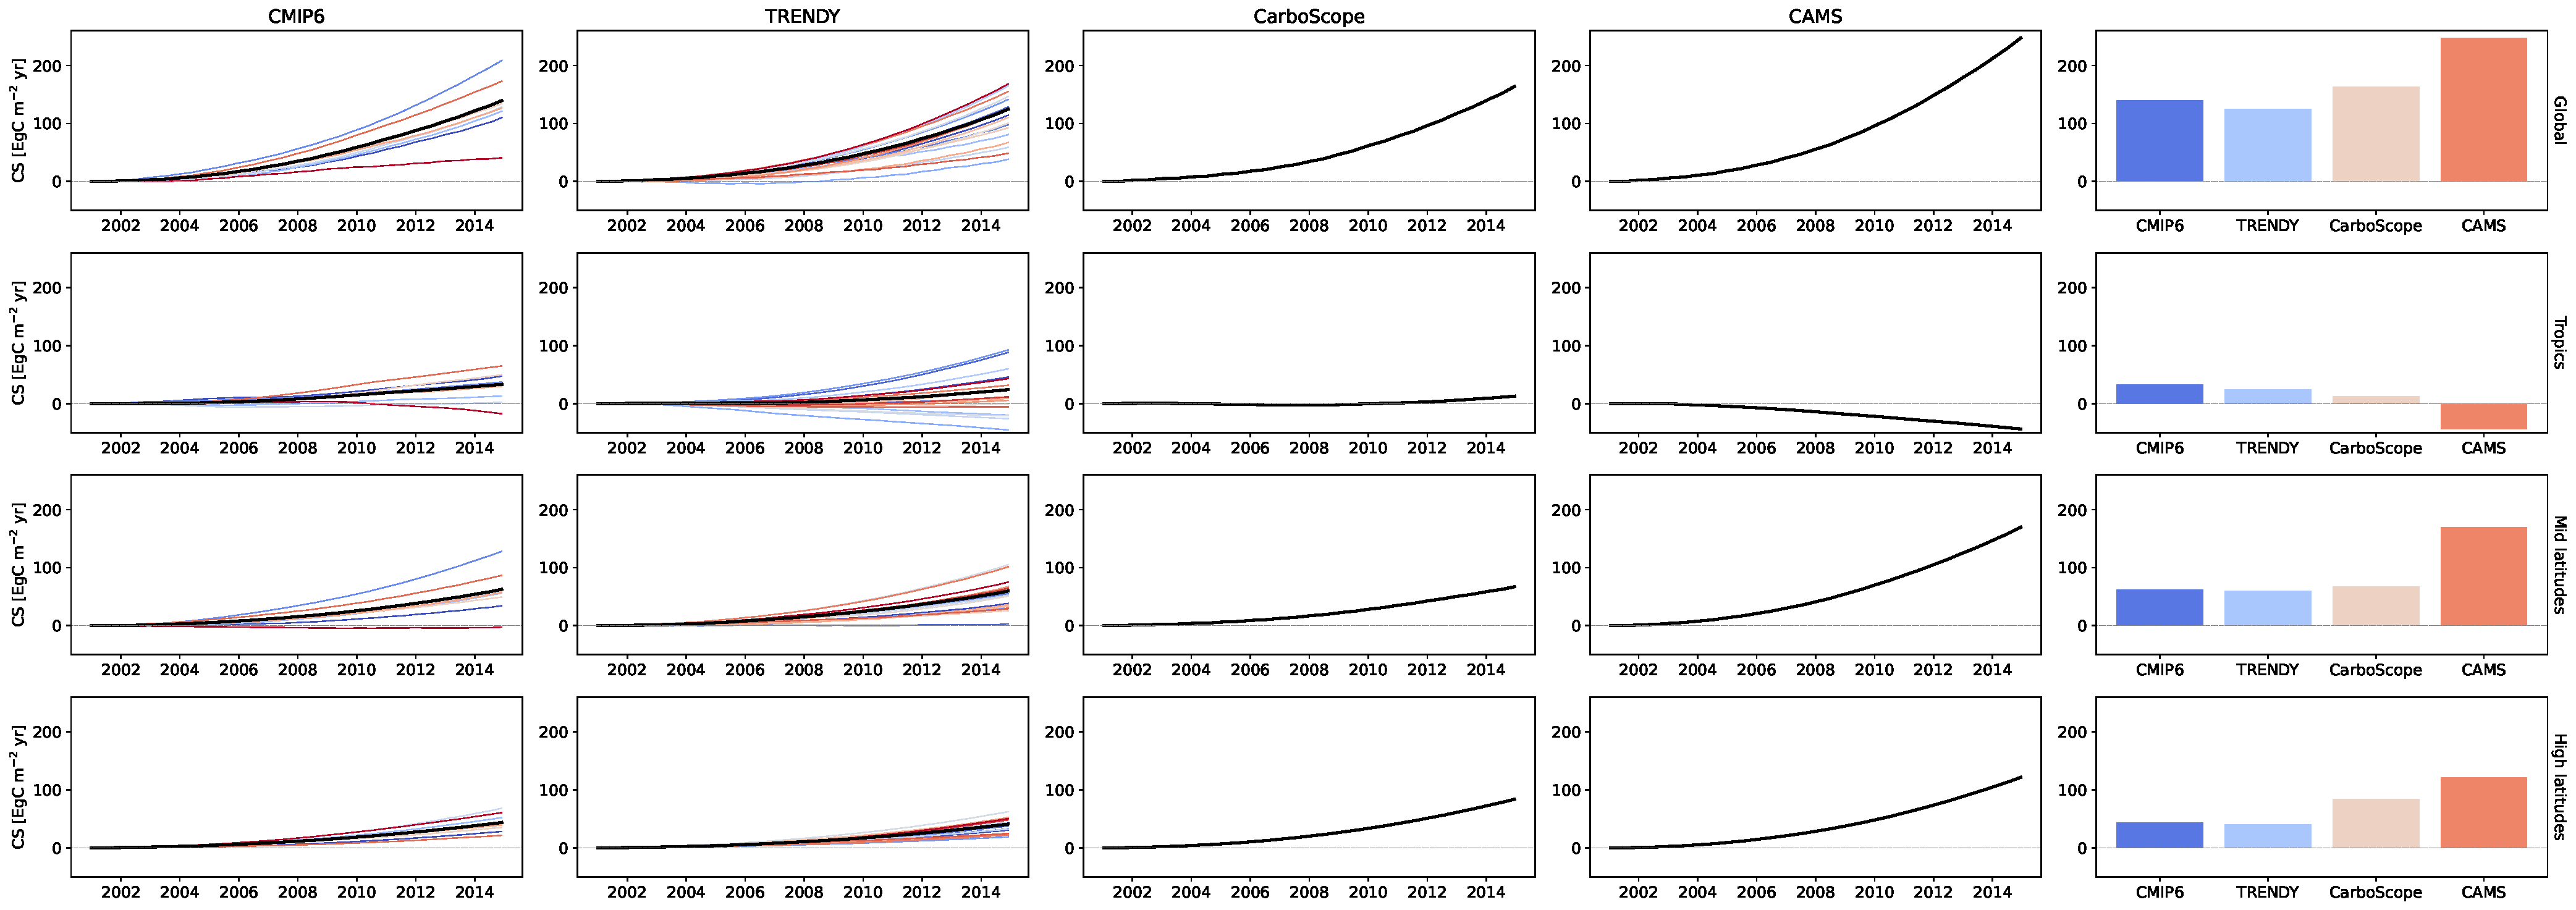
\includegraphics[width=1.0\linewidth]{Comparison_CS_temporal_NBP.pdf}
    \caption{Time accumulation of Carbon Sequestration (CS) of CMIP6 (1st vertical panel), TRENDY (2nd vertical panel), CarboScope (3rd vertical panel) and CAMS (4th vertical panel), and CS at the end of the period from 2001 to 2014 (right panel) calculated using NBP for global(1st horizontal panel), tropics (2nd horizontal panel), mid-latitudes (3rd horizontal panel), and high-latitudes zones (4th horizontal panel). Black lines in 1st and 2nd panels indicate the results using the ensemble of the models and bars for CMIP6 and TRENDY in the right panel correspond to their ensembles. The dotted lines indicate null values of CS.}
    \label{fig:TempCS_NBP}
\end{figure}

\end{document}



